\documentclass{standalone}

\usepackage{tikz}

\begin{document}
  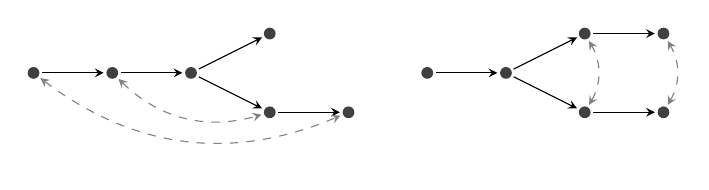
\begin{tikzpicture}
    \tikzstyle{v1} = [color=darkgray, circle, outer sep=1pt, fill, inner
      sep=1.5pt]
    \tikzstyle{v2} = [color=darkgray, circle, outer sep=1pt, fill, inner
      sep=3.0pt]
    \tikzstyle{e} = [->, >={stealth}] \tikzset{font=\tiny}

    % See fig-sigmaG-action-on-D5.tex
    \tikzstyle{a} = [color=gray, <->, dashed, >={stealth}]
    \tikzset{font=\tiny}

    \begin{scope}[shift={(0,0)}]
      \node[v1] (1) at (0, 0) {};
      \node[v1] (2) at (1, 0) {};
      \node[v1] (3) at (2, 0) {};
      \node[v1] (4) at (3, 0.5) {};
      \node[v1] (5) at (3, -0.50) {};
      \node[v1] (6) at (4, -0.50) {};
      \draw[e] (1) -- (2);
      \draw[e] (2) -- (3);
      \draw[e] (3) -- (4);
      \draw[e] (3) -- (5);
      \draw[e] (5) -- (6);
      \draw[a] (1) to[bend right] (6);
      \draw[a] (2) to[bend right] (5);
    \end{scope}

    \begin{scope}[shift={(5,0)}]
      \node[v1] (1) at (0,    0) {};
      \node[v1] (2) at (1,    0) {};
      \node[v1] (3) at (2, -0.5) {};
      \node[v1] (4) at (2,  0.5) {};
      \node[v1] (5) at (3, -0.5) {};
      \node[v1] (6) at (3,  0.5) {};
      \draw[e] (1) -- (2);
      \draw[e] (2) -- (3);
      \draw[e] (2) -- (4);
      \draw[e] (3) -- (5);
      \draw[e] (4) -- (6);
      \draw[a] (3) to[bend right] (4);
      \draw[a] (5) to[bend right] (6);
    \end{scope}
  \end{tikzpicture}
\end{document}
